%-------------------------------------------------------------------------
\section{Method}
Classic PRT  is a physically-based rendering method to accelerate on-line computations of the (simplified) \textit{Rendering Equation}:
\begin{align}
L_{\bm{s}}(\bm{\omega}_0 ) &= 
\int_{\Omega}   L_{\epsilon}(\bm{\omega}_i ) 
\underbrace{f(\bm{\omega}_i,\bm{\omega}_0) 
V(\bm{\omega}_i) H_N(\omega_i) }_{T(\bm{\omega}_i,\bm{\omega}_0) }
\,  \, d\bm{\omega}_i , 
\label{rendering equation PRT}
\end{align}
where $L_{\epsilon}$ accounts for all incoming radiance over the hemisphere, $f$  describes the surface reflectance properties $f$ (BRDF), $H_N$ is the \textit{Lambert's Law} and $V$ the \textit{Visibility Function} describing geometric information of the scene.\\
It precisely exploits the essence of static/non-deformable objects by uniquely determining the integrand $T(\bm{\omega}_i,\bm{\omega}_0)$ (called the \textbf{\textit{Transfer Function}} ), which contains the costly-to-compute  \textit{Visibility} term,
\begin{align*}
V :  \mathcal{S}  \times \Omega \rightarrow \{0,1\} \quad,
\end{align*}
for each surface point $\bm{s} \in \mathcal{S} \subset \mathbb{R}^3$ \cite{CohenBook, sloan2002precomputed}. 

Both functions $L_{\epsilon} $ and $T$  are projected onto a suitable set of orthonormal basis functions for faster evaluation, in our case \textit{Spherical Harmonics} (SH). \\
For $n$ number of SH bands and $l_i$, $t_i$ being the $i$-th SH coefficient of $L$ and $T$ respectively, the rendering equation \ref{rendering equation PRT} reduces to \cite{sloan2002precomputed}. 
\begin{align*}
L(\bm{\omega}_0 ) \approx \sum_{i}^{n^2} l_i \cdot t_i
\end{align*}
As mentioned above, our aim is to extend the PRT method to malleable and dynamic objects, but avoiding exhaustive pre-computations of every single \textit{Transfer Function} $T_i$ per shape query $S_i$ (with $i \in \{1,2,..., d\}$ ) that would imply enormous storage consumptions. \\
With this in mind, we propose a data-based model, a Convolutional Neural Network, to infer the Transfer Function $T_i$, more precisely the coefficients of its projection $t_j$'s, for any given shape query $S_i$. This makes the costly ray-casting computations superfluous and solves the abusive memory requirements, only requiring the storage of the network's parameters. 
\subsubsection*{Problem}
To this end, the network has to be fed with shape information. \\ 

% -------------- GEOMETRY IMAGE ----------------- 
\subsection{Object Reconstuction}
We chose a parametric approach called \textit{geometry Iimage } which translates the problem into a uniform grid on which standard CNNs can be applied \cite{gu2002geometry, sinha2016deep}. The parametrisation we chose is a harmonic mapping and the geometric data we transform into \textit{geomtry images} are vertex positions and normals (lets call them postion and normal image respectively)  (see Figure \ref{Fig: Method_Overview} picturing input and output of network)
\begin{figure}[H]
  \centering
    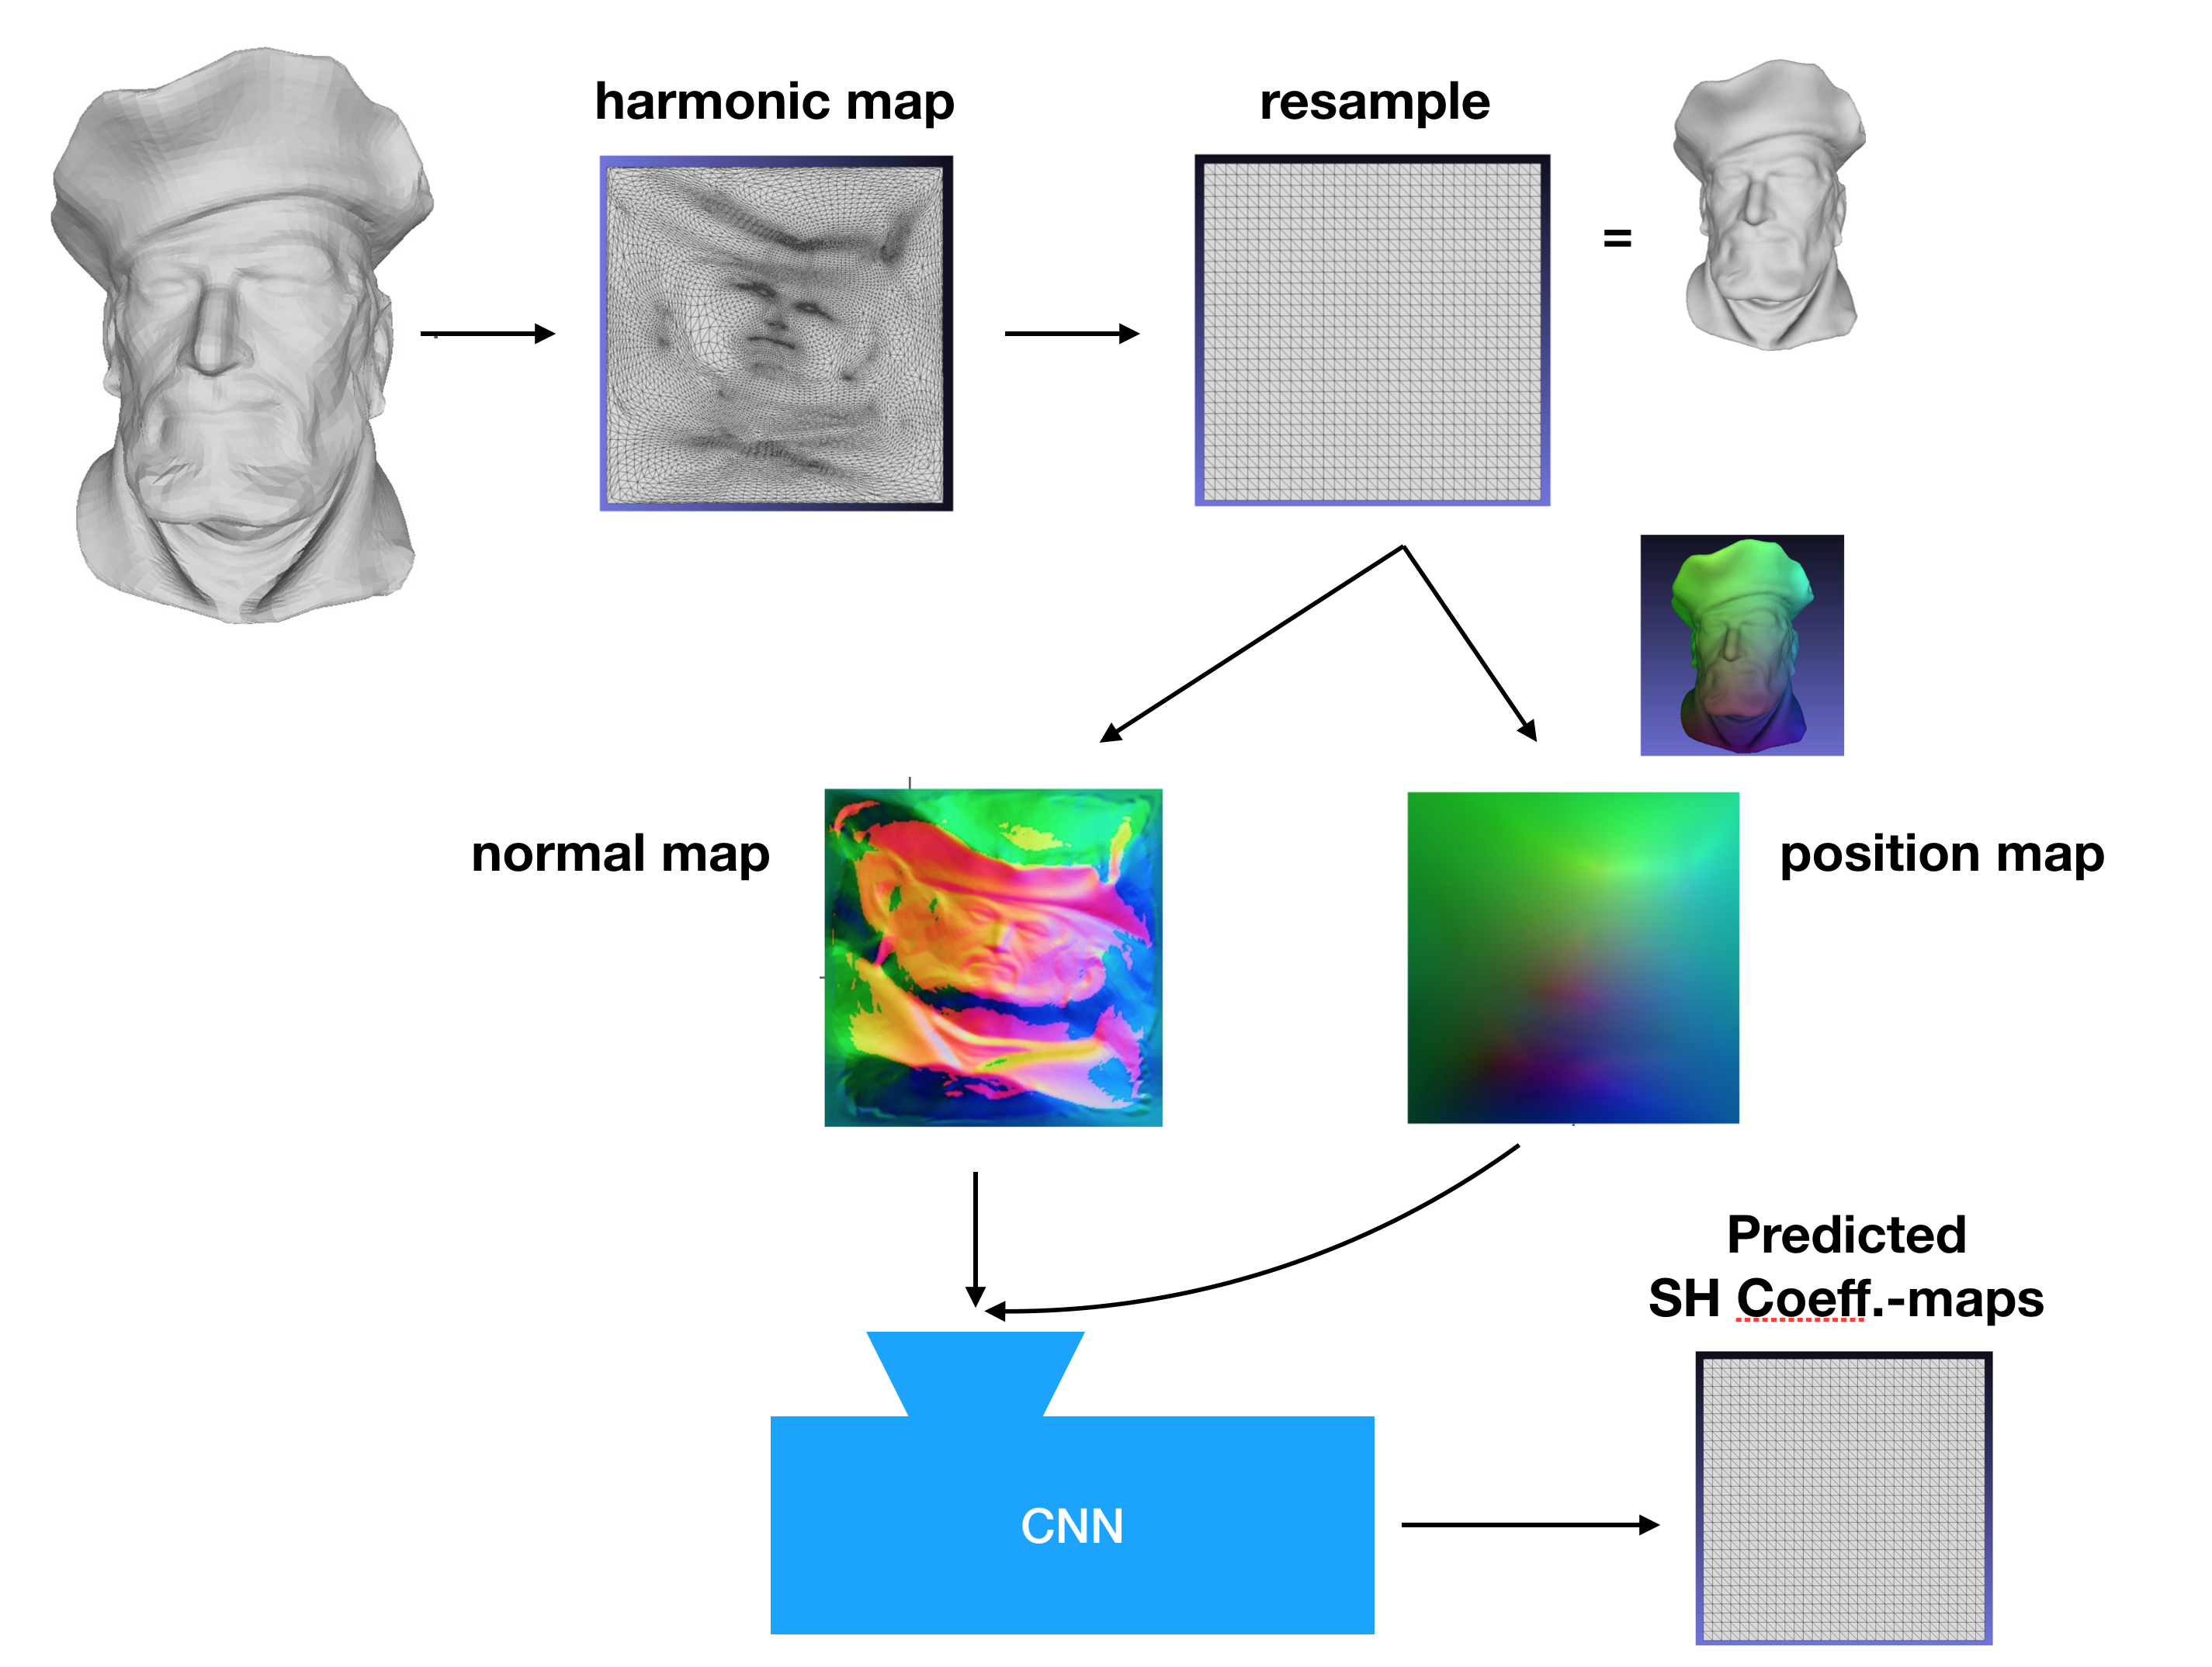
\includegraphics[width=0.5\textwidth]{Figures/Overview_method.pdf}
     \caption{Method Overview}
     \label{Fig: Method_Overview}
\end{figure}
\subsection{DPRT}
\subsubsection{Data}
We synthesise our training data by generating animations (such as cloth or faces, see example section) of deforming objects of 500 frames of duration. For each frame, a set
\begin{align*}
&\mathcal{D} = \{  \mathcal{P} , \mathcal{N} , \mathcal{T}\} 
\end{align*}
of position and normal images ($\mathcal{P}= \{ P_x , P_y, P_z \} $  and $\mathcal{N}= \{ N_x , N_y, N_z \} $) are created, where 
\begin{align*}
&P_i,N_i \in \mathbb{R}^{M \times M} ,
\quad
i \in \{x,y,z\}
\end{align*}
Besides, the a set of precomputed SH-Coefficients of the Transfer Function $\mathcal{T}= \{ T_0 , T_1, T_2, T_3..., T_{n^2} \} $  for the ground truth data...
\subsubsection{Network}



